%\newpage
\section{Snake}
\subsection*{Spielidee}
%\begin{wrapfigure}{r}{0.5\textwidth}
%	\begin{center}
%		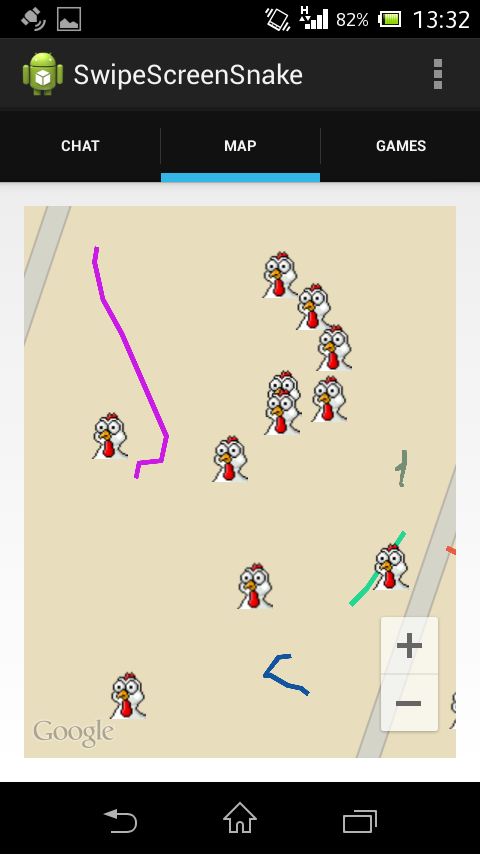
\includegraphics[width=0.48\textwidth]{5-Implementation_von_Beispielapps/5-1-Snake/Data/map_screen_snake.png}
%		\caption{Map-Screen von Snake}
%	\end{center}
%\end{wrapfigure}
Das erste Spiel, das wir umsetzen, ist das schon mehrfach erw�hnte Snake. Die Grundregeln von Snake sind der Mehrheit bekannt, da es auf nahezu allen Nokia-Handys der 90er Jahre mitgeliefert wurde.
In der implementierten Beispielapplikation verk�rpert jeder Spieler  eine Schlange. Der Kopf der virtuellen Schlange befindet sich auf der Spielerposition. Sobald der Spieler sich anf�ngt zu bewegen, zieht er einen Schwanz hinter sich her, der aus mehreren Gliedern besteht. Die L�nge des Schwanzes skaliert den Punktestand des Spielers. Der Spieler muss versuchen mit dem Kopf zuf�llig platzierte Bonusobjekte (H�hner/ Chickens) einzusammeln und es gleichzeitig vermeiden mit seinem eigenen Schwanz oder einer anderen Schlange zu kollidieren. Wenn dies dennoch geschieht wird der eigene Punktestand und die L�nge der Schlange zur�ckgesetzt. 
%Ziel des Spiels ist es schneller als die gegnerischen Schlangen eine einstellbare Anzahl von Punkten zu erreichen.

%Gibt doch gar keine Teams?


%Des weiteren l�sst sich das Spiel relativ leicht aus der virtuellen Landschaft in die physische Welt �bertragen, da die Steuerung nur auf der Bewegung des Kopfes der Schlange basiert. Dies kann in der Realit�t durch die Bewegung des Spielers selbst gesteuert werden. Wir haben uns f�r eine Mehrspieler Variante entschieden bei der in einem Spiel mehrere Zielpunkte (Chickens) gleichzeitig angezeigt werden, die beim (virtuellen) Einsammeln den Punktestand des Spielers erh�hen und die Schlange vergr��ern. Ziel des Spiels ist es schneller als die gegnerischen Schlangen eine einstellbare Anzahl von Punkten zu erreichen. Wenn man mit sich selbst oder einer anderen Schlange kollidiert wird der eigene Punktestand und die L�nge der Schlange zur�ckgesetzt.


\subsection*{Spiellogik}

%\subsubsection*{Server}
%Der implementierte Server arbeitet mit Java und ZeroMQ. Er �ffnet zwei Kommunikationskan�le mit dem Client. Der erste ist ein ZeroMQ-Request-Reply-Socket-Paar, �ber das die Endger�te Nachrichten an den Server senden. Der zweite ist ein Publish-Subscribe-Socket-Paar, �ber das die Nachrichten an Gruppen von Endger�ten weitergeleitet werden. Eine Nachricht besteht aus drei Teilen: einer Adresse, dem Nachrichtentyp und einem serialisierten Objekt vom Typ TransferObject (siehe Abbildung \ref{fig:transfer}). Die Adresse ist entweder die ID eines Spielers oder die ID einer Spielinstanz. Wir nutzen ZeroMQs Multipart-Message-Feature um diese Teile voneinander getrennt bei der Kommunikation zu �bermitteln. Der Server sendet eingehende Nachrichten an bestimmte Clients weiter. Das kann entweder ein einzelner Client, oder alle Clients die sich in einer Spielsession befinden, sein. Der Server kennt dabei den Zustand der einzelnen Spiele nicht. , Um mehrere Spielinstanzen gleichzeitig verwalten zu k�nnen, h�lt er aber eine Liste aller laufenden Spiele samt Informationen dar�ber, welcher Spieler an welchem Spiel teilnimmt. Wenn eine Nachricht vom Typ \glqq create\_game\grqq empfangen wird tr�gt der Server die ID des Spiels in eine Liste ein. Diese Liste wird einem Client gesendet wenn er sie �ber eine entsprechende Nachricht anfragt.
%
Der Server dient bei dieser Implementation nur zur Weiterleitung der Nachrichten.

%\begin{figure}
%\begin{center}
%    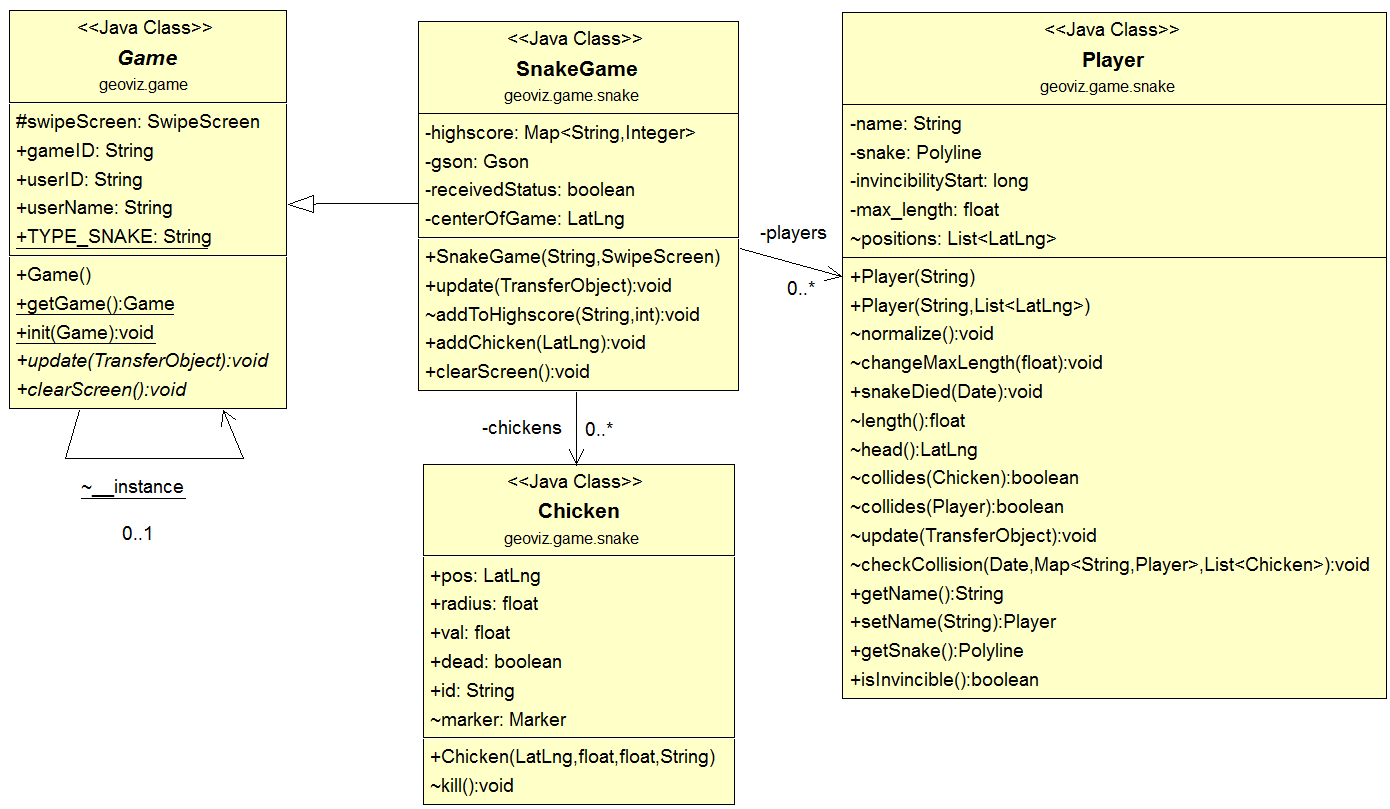
\includegraphics[width=1\textwidth]{img/snake.png}
%\end{center}
%
%     \caption{UML-Diagramm zur Spiellogik}
%     \label{fig:snake}
%\end{figure}

%\subsubsection*{Client}
%Unsere Android-Applikation besteht aus drei Fragmenten zwischen denen man durch Wischen wechseln kann. Das erste Fragment ist ein Chat �ber den Spieler Textnachrichten an ihre Mitspieler im gleichen Spiel senden k�nnen.
%Das zweite Fragment ist die Karte auf der wir unser Spiel darstellen.  
%F�r die Darstellung der Karte verwenden wir GoogleMaps. 
%Im dritten Fragment kann ein Spieler eine neue Spielinstanz erstellen oder einem bereits laufendem Spiel beitreten. Die Liste der momentan laufenden Spiele wird per Knopfdruck vom Server abgefragt. Wenn man einer laufenden Session beitritt wird �ber den Server eine Anfrage des aktuellen Status des Spiels an alle momentanen Mitspieler gesendet, welche den Zustand des Spiels alle an den anfragenden Client zur�ck senden. Dieser beachtet nur die erste Nachricht und verwirft den Rest.
%Des weiteren l�uft ein LocationClient, welcher immer die aktuelle Position als Nachricht an alle Spieler der selben Spielinstanz weiterschickt. 
%\begin{figure}
%	\begin{center}
%		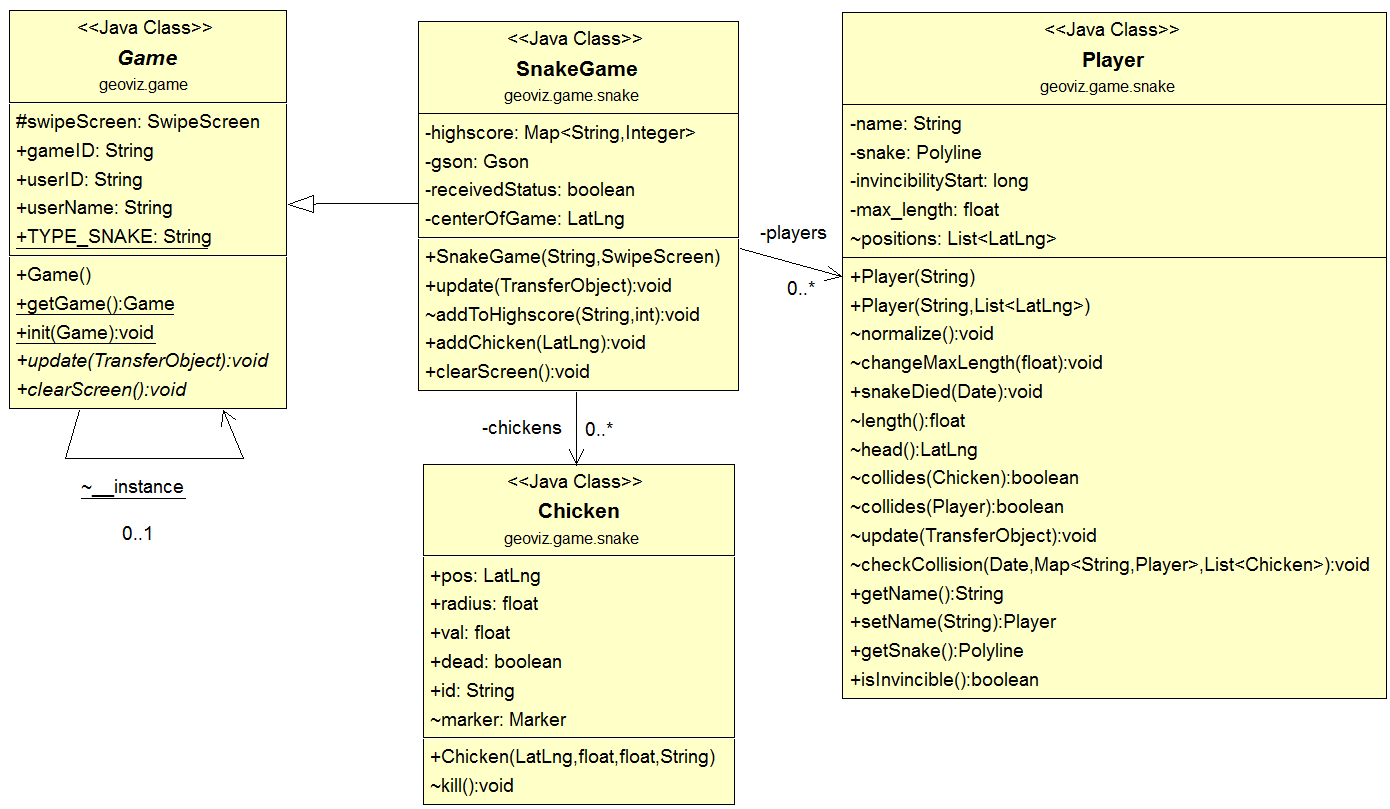
\includegraphics[width=1\textwidth]{img/snake.png}
%	\end{center}
%	
%	\caption{UML-Diagramm zur Spiellogik}
%	\label{fig:snake}
%\end{figure}


\paragraph{Darstellung der Schlange:}
Die Schlange wird als Polygonzug (eine Menge von Punkten zwischen denen Linien gezeichnet werden) dargestellt. Hierf�r wird eine Polyline\footnote{\url{https://developers.google.com/android/reference/com/google/android/gms/maps/model/Polyline}} verwendet. Der Polygonzug eines jeden Spielers hat eine bestimmte L�nge, die von den erreichten Punkten abh�ngt. Es wird jeweils die neue Position des Spielers am Anfang des Polygonzugs (Kopf)  eingetragen. Entsprechend der erreichten L�nge, werden die letzten Punkte gel�scht.

\paragraph{Objekte aufsammeln:}
Jeder Client �berpr�ft nur f�r sich selbst, ob er nahe genug an einem Objekt ist, um diesen aufzusammeln und sendet diese Information weiter an alle Mitspieler inklusive sich selbst. Erst beim Empfang dieser Nachricht wird die L�nge der Schlange ver�ndert und das Objekt von der Karte entfernt.
Die Objekte werden zuf�llig in der N�he der Spieler erzeugt. Wenn sich die Anzahl durch einsammeln reduziert, werden neue Objekte generiert.

\paragraph{Kollision:}
Die Kollision wird durch Abstandsmessung realisiert (siehe Abschnitt \ref{abstandsmessung}). Hierbei wird bei jedem Positionsupdate die Distanz zu allen kollisionsrelevanten Punkten (Eigener Schwanz, komplette Schlangen anderer Spieler) gemessen. Unterschreitet die Distanz einen gewissen Wert, wird eine Kollision ausgel�st. Aufgrund der schwankenden Positionsupdatefrequenz und Bewegungsgeschwindigkeit der Spieler, wird bei der Eigenkollision die ersten vier Meter der Schlange ignoriert. Bei einem Spielstart oder dem "`Tod"' der Schlange wird jegliche Kollision f�r einen kurzen Zeitraum deaktiviert.





